% F2 method diagram: the attention logit as a Fourier series over the offset, and the three knobs.
% Build: ~/.local/bin/tectonic -X compile f2_method.tex   -> f2_method.pdf, 5.5 in wide (final print size).
% Every number drawn here (wavelengths, band gains, ln tau, summed curves) comes from
% f2_method_data.tex, written by f2_method_data.py from the run sidecars.
% Colors and names follow DESIGN_NOTES.md and crope_style.py; notation follows sec/background.tex.
\documentclass[border=0pt]{standalone}
\usepackage[T1]{fontenc}
\usepackage{tgheros}
\renewcommand\familydefault{\sfdefault}
\usepackage{newtxsf}
% keep every sub- and superscript at or above 6.4 pt (PDF points) at native size (the paper includes F2 at 0.86 linewidth)
\DeclareMathSizes{6.5}{6.5}{6.45}{6.45}\DeclareMathSizes{7}{7}{6.45}{6.45}
\DeclareMathSizes{8}{8}{6.45}{6.45}\DeclareMathSizes{9}{9}{6.45}{6.45}
\usepackage{tikz}
\usetikzlibrary{arrows.meta, calc, shapes.geometric}
% Generated by f2_method_data.py; do not edit by hand.
% prompt row 8 (a4k_eval_4096_880657115260655727), seed 0, step 14 of 28, sigma = 0.7595
% SEGA base b' = 155716.5; ln tau = 0.22181
\def\FtwoLnTau{0.22181}
\def\FtwoSigma{0.76}
\def\FtwoStep{14}
% row index / j / T_j at b' / T_j at b / lambda SEGA / lambda Constancy-TM
\def\FtwoStack{0/6/81.437/45.219/0.25372/0.17438, 1/8/191.295/87.305/0.28474/-0.08997, 2/10/449.350/168.559/0.24445/0.22181, 3/12/1055.519/325.436/0.26387/0.22181}
\def\FtwoTnA{81.437}\def\FtwoToA{45.219}
\def\FtwoTnB{191.295}\def\FtwoToB{87.305}
\def\FtwoTnC{449.350}\def\FtwoToC{168.559}
\def\FtwoTnD{1055.519}\def\FtwoToD{325.436}
\def\FtwoBaseBand{8}
\def\FtwoBaseTnew{191.295}
\def\FtwoBaseTold{87.305}
% all 28 width-axis bands: j / lambda SEGA / lambda Constancy-TM
\def\FtwoAll{0/0.29416/0.22178, 1/0.24969/0.22087, 2/0.27982/0.22269, 3/0.27986/0.22328, 4/0.23412/0.22357, 5/0.27951/0.20350, 6/0.25372/0.17438, 7/0.23964/0.10339, 8/0.28474/-0.08997, 9/0.30716/0.22181, 10/0.24445/0.22181, 11/0.23620/0.22181, 12/0.26387/0.22181, 13/0.24810/0.22181, 14/0.24679/0.22181, 15/0.27270/0.22181, 16/0.25988/0.22181, 17/0.24741/0.22181, 18/0.25603/0.22181, 19/0.28085/0.22181, 20/0.24402/0.22181, 21/0.23864/0.22181, 22/0.18069/0.22181, 23/0.23986/0.22181, 24/0.15551/0.22181, 25/0.06384/0.22181, 26/0.00000/0.22181, 27/0.00000/0.22181}


% ---------------------------------------------------------------- palette (crope_style.py)
\definecolor{ink}{HTML}{1F2329}
\definecolor{ink2}{HTML}{5B6270}
\definecolor{rule}{HTML}{C9CDD3}
\definecolor{panel}{HTML}{F3F4F6}
\definecolor{gridc}{HTML}{E3E5E8}
\definecolor{cobalt}{HTML}{1F4E8C}
\definecolor{sky}{HTML}{7EA9D9}
\definecolor{stone}{HTML}{9A9A9A}
\definecolor{terra}{HTML}{D35F3A}

% ---------------------------------------------------------------- type scale (print size)
\newcommand\fsLetter{\fontsize{9}{10}\selectfont\bfseries}
\newcommand\fsEq{\fontsize{8}{9.6}\selectfont}
\newcommand\fsMain{\fontsize{7}{8.4}\selectfont}
\newcommand\fsSmall{\fontsize{6.5}{7.6}\selectfont}
% equation highlights: same height for every symbol
\newcommand\hl[2]{{\setlength\fboxsep{0.6pt}\colorbox{#1}{$#2\vphantom{bg}$}}}
\newcommand\hlg[1]{\tikz[baseline=(h.base)]\node[left color=cobalt!24, right color=terra!26,
  inner xsep=0.6pt, inner ysep=0.6pt] (h) {$#1\vphantom{bg}$};}
% knob note: hierarchy (italic) over role
\newcommand\knobnote[2]{{\fsSmall\color{ink2}\begin{tabular}{@{}l@{}}\textit{#1}\\[-0.4mm]#2\end{tabular}}}

\begin{document}
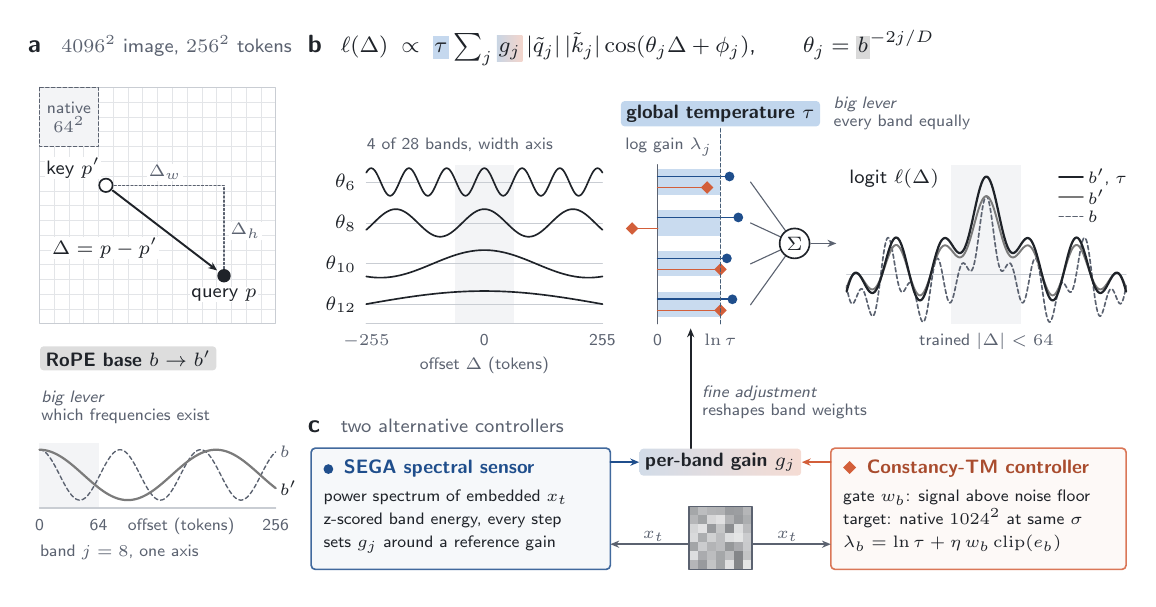
\begin{tikzpicture}[x=1mm, y=1mm, line cap=round, line join=round,
  >={Stealth[length=3.2pt, width=2.6pt]},
  every node/.style={inner sep=0pt, text=ink},
  lbl/.style={font=\fsMain},
  sml/.style={font=\fsSmall, text=ink2},
  halo/.style={fill=white, inner sep=0.5pt},
  pill/.style={fill=#1, rounded corners=1.3pt, inner xsep=2.0pt, inner ysep=1.45pt,
    font=\fsMain\bfseries},
  ctrl/.style={draw=#1!85, fill=#1!4, rounded corners=1.5pt, line width=0.6pt},
  wave/.style={ink, line width=0.6pt},
  flow/.style={->, ink2, line width=0.6pt},
  edgelbl/.style={font=\fsSmall, text=ink2, inner sep=0.6pt},
]
\path[use as bounding box] (0,0) rectangle (139.7,70);

% ================================================================= a: offset on the token grid
\node[anchor=base west, font=\fsLetter] at (0,66.8) {a};
\node[anchor=base west, lbl, text=ink2] at (4.2,66.8) {$4096^2$ image, $256^2$ tokens};
\def\gx{1.5}\def\gy{32.4}\def\gs{30}
\foreach \i in {1,...,15} {
  \draw[gridc, line width=0.25pt] (\gx+\i*\gs/16,\gy) -- ++(0,\gs);
  \draw[gridc, line width=0.25pt] (\gx,\gy+\i*\gs/16) -- ++(\gs,0);
}
\draw[rule, line width=0.5pt] (\gx,\gy) rectangle ++(\gs,\gs);
% native 64^2 extent: one quarter per side
\fill[panel] (\gx,\gy+\gs) rectangle ++(\gs/4,-\gs/4);
\draw[ink2, line width=0.5pt, dash pattern=on 1.2pt off 0.9pt] (\gx,\gy+\gs) rectangle ++(\gs/4,-\gs/4);
\node[sml, align=center, font=\fontsize{6.5}{6.9}\selectfont] at (\gx+\gs/8,\gy+\gs-\gs/8) {native\\$64^2$};
% key p' and query p (token coordinates on the 256 grid)
\coordinate (k) at (\gx+72/256*\gs, \gy+150/256*\gs);
\coordinate (q) at (\gx+200/256*\gs, \gy+52/256*\gs);
\draw[ink2, line width=0.4pt, dash pattern=on 0.8pt off 0.7pt] (k) -- (k-|q) -- (q);
\draw[->, ink, line width=0.7pt, shorten <=1.1mm, shorten >=1.1mm] (k) -- (q);
\fill[ink] (q) circle (0.85);
\draw[ink, fill=white, line width=0.6pt] (k) circle (0.85);
\node[lbl, halo, anchor=south east] at ($(k)+(-0.5,0.7)$) {key $p'$};
\node[lbl, halo, anchor=north] at ($(q)+(0,-1.4)$) {query $p$};
\node[sml, halo, anchor=south] at ($(k)!0.5!(k-|q)+(0,0.5)$) {$\Delta_w$};
\node[sml, halo, anchor=west] at ($(k-|q)!0.5!(q)+(0.6,0)$) {$\Delta_h$};
\node[lbl, halo, anchor=north east] at ($(k)!0.5!(q)+(-0.7,-0.7)$) {$\Delta=p-p'$};

% base knob: band j along one axis under the native base b and SEGA's base b'
\node[pill=stone!34, anchor=north west] (base) at (\gx,29.6) {RoPE base $b\to b'$};
\node[anchor=north west, halo] at (\gx,24.5) {\knobnote{big lever}{which frequencies exist}};
\def\my{13.2}\def\ma{3.2}
\fill[panel] (\gx,9.0) rectangle (\gx+\gs/4,\my+\ma+0.8);
\draw[rule, line width=0.4pt] (\gx,9.0) -- ++(\gs,0);
\draw[ink2, line width=0.5pt, dash pattern=on 1.5pt off 1pt]
  plot[domain=0:256, samples=181] ({\gx+\gs*\x/256},{\my+\ma*cos(\x*(360/\FtwoBaseTold))});
\draw[stone!80!black, line width=0.8pt]
  plot[domain=0:256, samples=121] ({\gx+\gs*\x/256},{\my+\ma*cos(\x*(360/\FtwoBaseTnew))});
\node[sml, anchor=west] at (\gx+\gs+0.5,{\my+\ma*cos(256*(360/\FtwoBaseTold))}) {$b$};
\node[sml, anchor=west, text=ink] at (\gx+\gs+0.5,{\my+\ma*cos(256*(360/\FtwoBaseTnew))}) {$b'$};
\node[sml, anchor=base] at (\gx,6.2) {0};
\node[sml, anchor=base] at (\gx+\gs/4,6.2) {64};
\node[sml, anchor=base] at (\gx+\gs,6.2) {256};
\node[sml, anchor=base] at (\gx+\gs*0.6,6.2) {offset (tokens)};
\node[sml, anchor=base west] at (\gx,2.9) {band $j=\FtwoBaseBand$, one axis};

% ================================================================= b: logit as a Fourier series in the offset
\node[anchor=base west, font=\fsLetter] at (35.5,66.8) {b};
\node[anchor=base west, font=\fsEq] at (39.7,66.8)
  {$\ell(\Delta)\;\propto\;\hl{sky!45}{\tau}\sum_j \hlg{g_j}\,|\tilde q_j|\,|\tilde k_j|\cos(\theta_j\Delta+\phi_j)$,\qquad
    $\theta_j=\hl{stone!38}{b}^{-2j/D}$};

\def\wx{43}\def\ww{30}\def\wc{58}\def\amp{1.75}
\def\ya{50.4}\def\ysp{5.2}\def\yb{32.4}\def\yt{52.6}
\node[sml, anchor=base west] at (\wx,54.5) {4 of 28 bands, width axis};
\node[sml, anchor=base east] at (87,54.5) {log gain $\lambda_j$};
\fill[panel] (\wc-\ww/8,\yb) rectangle (\wc+\ww/8,\yt);
\foreach \k/\j/\Tn/\To/\ls/\lc in \FtwoStack {
  \pgfmathsetmacro\yy{\ya-\k*\ysp}
  \draw[rule, line width=0.3pt] (\wx,\yy) -- ++(\ww,0);
  \draw[wave] plot[domain=-255:255, samples=241] ({\wc+\ww/2*\x/255},{\yy+\amp*cos(\x*(360/\Tn))});
  \node[lbl, anchor=east] at (\wx-1.2,\yy) {$\theta_{\j}$};
}
\draw[rule, line width=0.4pt] (\wx,\yb) -- ++(\ww,0);
\node[sml, anchor=base] at (\wx,29.6) {$-255$};
\node[sml, anchor=base] at (\wc,29.6) {0};
\node[sml, anchor=base] at (\wx+\ww,29.6) {255};
\node[sml, anchor=base] at (\wc,26.6) {offset $\Delta$ (tokens)};

% band log gains lambda_j = ln(tau g_j): sky bar = ln tau (identical for every band);
% lollipops = real per-band values (circle SEGA, diamond Constancy-TM)
\def\fz{80}\def\fk{36}
\pgfmathsetmacro\ft{\fz+\fk*\FtwoLnTau}
\draw[ink2, line width=0.4pt] (\fz,\yb) -- (\fz,\yt);
\foreach \k/\j/\Tn/\To/\ls/\lc in \FtwoStack {
  \pgfmathsetmacro\yy{\ya-\k*\ysp}
  \fill[sky!42] (\fz,\yy-1.6) rectangle (\ft,\yy+1.6);
  \draw[cobalt, line width=0.6pt] (\fz,\yy+0.7) -- ({\fz+\fk*\ls},\yy+0.7);
  \draw[terra, line width=0.6pt] (\fz,\yy-0.7) -- ({\fz+\fk*\lc},\yy-0.7);
  \fill[cobalt] ({\fz+\fk*\ls},\yy+0.7) circle (0.62);
  \node[diamond, fill=terra, minimum size=1.65mm] at ({\fz+\fk*\lc},\yy-0.7) {};
}
\draw[sky!55!black, line width=0.5pt, dash pattern=on 1.2pt off 0.9pt] (\ft,\yb) -- (\ft,57.4);
\node[sml, anchor=base] at (\fz,29.6) {0};
\node[sml, anchor=base] at (\ft,29.6) {$\ln\tau$};
\node[pill=sky!48, anchor=south] (temp) at (\ft,57.4) {global temperature $\tau$};
\node[anchor=west] at ($(temp.east)+(1.6,0)$) {\knobnote{big lever}{every band equally}};

% summing junction and output logit
\coordinate (sig) at (97.4,{\ya-1.5*\ysp});
\foreach \k in {0,...,3} {
  \pgfmathsetmacro\yy{\ya-\k*\ysp}
  \draw[ink2, line width=0.4pt] (91.8,\yy) -- ($(sig)!1.9mm!(91.8,\yy)$);
}
\draw[ink, line width=0.6pt, fill=white] (sig) circle (1.9);
\node[font=\fsMain] at (sig) {$\Sigma$};
\draw[flow] ($(sig)+(2.1,0)$) -- ($(sig)+(5.3,0)$);
\def\lx{104}\def\lw{35.5}\def\lc{121.75}\def\lz{38.6}\def\lu{2.5}
\fill[panel] (\lc-\lw/8,\yb) rectangle (\lc+\lw/8,\yt);
\draw[rule, line width=0.4pt] (\lx,\lz) -- ++(\lw,0);
\draw[ink2, line width=0.6pt, dash pattern=on 1.5pt off 1pt] plot[domain=-255:255, samples=401]
  ({\lc+\lw/2*\x/255},{\lz+\lu*(cos(\x*(360/\FtwoToA))+cos(\x*(360/\FtwoToB))+cos(\x*(360/\FtwoToC))+cos(\x*(360/\FtwoToD)))});
\draw[stone!80!black, line width=0.7pt] plot[domain=-255:255, samples=301]
  ({\lc+\lw/2*\x/255},{\lz+\lu*(cos(\x*(360/\FtwoTnA))+cos(\x*(360/\FtwoTnB))+cos(\x*(360/\FtwoTnC))+cos(\x*(360/\FtwoTnD)))});
\draw[ink, line width=0.8pt] plot[domain=-255:255, samples=301]
  ({\lc+\lw/2*\x/255},{\lz+\lu*exp(\FtwoLnTau)*(cos(\x*(360/\FtwoTnA))+cos(\x*(360/\FtwoTnB))+cos(\x*(360/\FtwoTnC))+cos(\x*(360/\FtwoTnD)))});
\node[lbl, anchor=base west] at (\lx+0.3,50.2) {logit $\ell(\Delta)$};
\begin{scope}[shift={(131.0,51.0)}]
  \draw[ink, line width=0.8pt] (0,0) -- (3,0);                  \node[sml, anchor=west, text=ink] at (3.6,0) {$b'$, $\tau$};
  \draw[stone!80!black, line width=0.7pt] (0,-2.5) -- (3,-2.5); \node[sml, anchor=west, text=ink] at (3.6,-2.5) {$b'$};
  \draw[ink2, line width=0.6pt, dash pattern=on 1.5pt off 1pt] (0,-5) -- (3,-5); \node[sml, anchor=west, text=ink] at (3.6,-5) {$b$};
\end{scope}
\node[sml, anchor=base] at (\lc,29.6) {trained $|\Delta|<64$};

% ================================================================= c: per-band controllers
\node[anchor=base west, font=\fsLetter] at (35.5,18.6) {c};
\node[anchor=base west, lbl, text=ink2] at (39.7,18.6) {two alternative controllers};
\def\cy{1.2}\def\ch{15.4}
\node[anchor=north, left color=cobalt!20, right color=terra!22, rounded corners=1.3pt,
      inner xsep=2.0pt, inner ysep=1.45pt, font=\fsMain\bfseries]
  (alloc) at (\ft,\cy+\ch) {per-band gain $g_j$};
\draw[->, ink, line width=0.6pt] (alloc.north -| 84.2,0) -- (84.2,\yb-0.6);
\node[anchor=west] at (85.6,22.4) {\knobnote{fine adjustment}{reshapes band weights}};

% latent x_t (noise texture icon), read by both controllers
\begin{scope}[shift={(\ft-4,\cy)}]
  \pgfmathsetseed{11}
  \foreach \i in {0,...,6} { \foreach \j in {0,...,6} {
    \pgfmathsetmacro\g{12+int(random(0,44))}
    \fill[ink!\g] (\i*8/7,\j*8/7) rectangle ++(8/7,8/7);
  }}
  \draw[ink2, line width=0.4pt] (0,0) rectangle (8,8);
\end{scope}

\draw[ctrl=cobalt] (36,\cy) rectangle (74,\cy+\ch);
\node[anchor=north west, font=\fsMain\bfseries, text=cobalt] at (37.5,\cy+\ch-1.5) {\tikz\fill[cobalt] (0,0) circle (0.62mm);\, SEGA spectral sensor};
\node[anchor=north west, sml, text=ink, align=left] at (37.5,\cy+\ch-5.3)
  {power spectrum of embedded $x_t$\\[0.2mm] z-scored band energy, every step\\[0.2mm] sets $g_j$ around a reference gain};
\draw[ctrl=terra] (102,\cy) rectangle (139.5,\cy+\ch);
\node[anchor=north west, font=\fsMain\bfseries, text=terra!80!black] at (103.5,\cy+\ch-1.5) {\tikz\node[diamond, fill=terra, minimum size=1.7mm]{};\, Constancy-TM controller};
\node[anchor=north west, sml, text=ink, align=left] at (103.5,\cy+\ch-5.3)
  {gate $w_b$: signal above noise floor\\[0.2mm] target: native $1024^2$ at same $\sigma$\\[0.2mm]
   $\lambda_b=\ln\tau+\eta\,w_b\,\mathrm{clip}(e_b)$};
% wiring: x_t out to both controllers (bottom), g_j back in to the chip (top)
\draw[flow] (\ft-4,\cy+3.2) -- node[edgelbl, above, pos=0.45] {$x_t$} (74,\cy+3.2);
\draw[flow] (\ft+4,\cy+3.2) -- node[edgelbl, above, pos=0.45] {$x_t$} (102,\cy+3.2);
\draw[->, cobalt, line width=0.6pt] (74,0 |- alloc.west) -- (alloc.west);
\draw[->, terra, line width=0.6pt] (102,0 |- alloc.east) -- (alloc.east);
\end{tikzpicture}
\end{document}
